


%_______________
\section{Review exercises}

% 1

\eoce{\qt{GPA and study hours\label{gpa_study_hours}} A survey was conducted on 193 
Duke University undergraduates who took an introductory statistics course in 
2012. Among many other questions, this survey asked them about their GPA, which 
can range between 0 and 4 points, and the number of hours they spent studying 
per week. The scatterplot below displays the relationship between these two 
variables.

\noindent\begin{minipage}[c]{0.44\textwidth}
\begin{parts}
\item What is the explanatory variable and what is the response variable?
\item Describe the relationship between the two variables. Make sure to discuss 
unusual observations, if any.
\item Is this an experiment or an observational study?
\item Can we conclude that studying longer hours leads to higher GPAs?
\end{parts}
\end{minipage}
\begin{minipage}[c]{0.55\textwidth}
\begin{center}
\includegraphics[width = 0.78\textwidth]{ch_intro_to_data/figures/eoce/gpa_study_hours/gpa_study_hours_scatterplot.pdf}
\end{center}
\end{minipage}
}{}

% 2

\eoce{\qt{City council survey\label{city_council_survey}} A city council has requested a 
household survey be conducted in a suburban area of their city. The area is broken 
into many distinct and unique neighborhoods, some including large homes, some with 
only apartments, and others a diverse mixture of housing structures. Identify the 
sampling methods described below, and comment on whether or not you think they 
would be effective in this setting.
\begin{parts}
\item Randomly sample 50 households from the city.
\item Divide the city into neighborhoods, and sample 20 households from each 
neighborhood.
\item Divide the city into neighborhoods, randomly sample 10 neighborhoods, 
and sample all households from those neighborhoods.
\item Divide the city into neighborhoods, randomly sample 10 neighborhoods, 
and then randomly sample 20 households from those neighborhoods.
\item Sample the 200 households closest to the city council offices.
\end{parts}
}{}

% 3

\eoce{\qt{Flawed reasoning\label{flawed_reasoning}} Identify the flaw(s) in reasoning 
in the following scenarios. Explain what the individuals in the study should 
have done differently if they wanted to make such strong conclusions.
\begin{parts}
\item Students at an elementary school are given a questionnaire that they 
are asked to return after their parents have completed it. One of the questions 
asked is, ``Do you find that your work schedule makes it difficult for you to 
spend time with your kids after school?" Of the parents who replied, 85\% said 
``no". Based on these results, the school officials conclude that a great 
majority of the parents have no difficulty spending time with their kids 
after school.
\item A survey is conducted on a simple random sample of 1,000 women who 
recently gave birth, asking them about whether or not they smoked during 
pregnancy. A follow-up survey asking if the children have respiratory problems 
is conducted 3 years later, however, only 567 of these women are reached at the 
same address. The researcher reports that these 567 women are representative 
of all mothers.
\item An orthopedist administers a questionnaire to 30 of his patients who do 
not have any joint problems and finds that 20 of them regularly go running. 
He concludes that running decreases the risk of joint problems.
\end{parts}
}{}

% 4

\eoce{\qt{Income and education in US counties\label{income_education_county}} 
The scatterplot below shows the relationship between per capita income 
(in thousands of dollars) and percent of population with a bachelor's 
degree in 3,143 counties in the US in 2010.

\noindent\begin{minipage}[c]{0.44\textwidth}
\begin{parts}
\item What are the explanatory and response variables?
\item Describe the relationship between the two variables. Make sure to discuss 
unusual observations, if any.
\item Can we conclude that having a bachelor's degree increases one's income?
\end{parts}\vspace{8mm}
\end{minipage}
\begin{minipage}[c]{0.55\textwidth}
\begin{center}
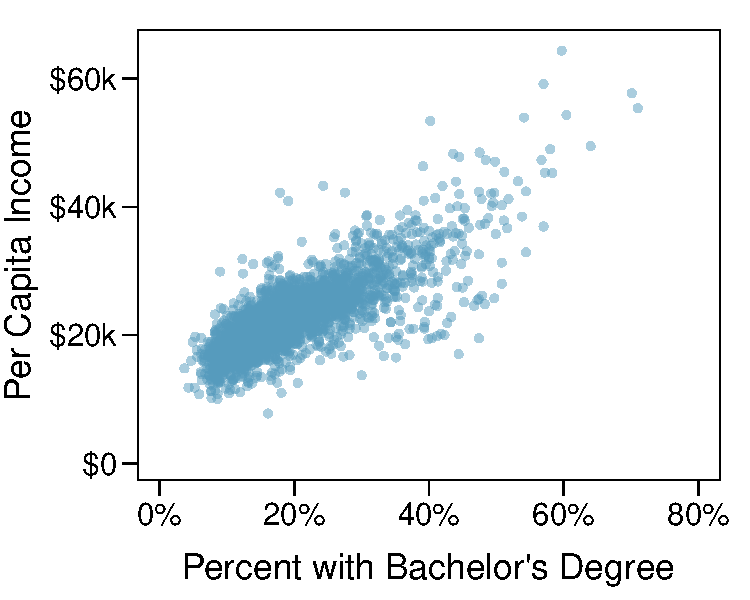
\includegraphics[width = 0.78\textwidth]{ch_intro_to_data/figures/eoce/county_income_education/county_income_education_scatterplot.pdf}
\end{center}
\end{minipage}
}{}

% 5

\eoce{\qt[?]{Eat better, feel better\label{eat_better_feel_better}} In a public health 
study on the effects of consumption of fruits and vegetables on psychological 
well-being in young adults, participants were randomly assigned to three 
groups: (1) diet-as-usual, (2) an ecological momentary intervention involving 
text message reminders to increase their fruits and vegetable consumption plus 
a voucher to purchase them, or (3) a fruit and vegetable intervention in 
which participants were given two additional daily servings of fresh fruits and 
vegetables to consume on top of their normal diet. Participants were asked to 
report on their psychological well-being with a nightly survey they took on 
their smart phones. Participants were student volunteers at the University of 
Otago, New Zealand. At the end of the 14-day study, only participants in the third 
group improvements to their psychological well-being across the 14-days relative 
to the other groups.\footfullcite{conner2017let}
\begin{parts}
\item What type of study is this?
\item Identify the explanatory and response variables.
\item Comment on whether the results of the study can be generalized to 
the population.
\item Comment on whether the results of the study can be used to establish 
causal relationships.
\item A newspaper article reporting on the study states "The results of this 
study provide proof that giving young adults fresh fruit and vegetables to eat 
can have psychological benefits, even over a brief period of time." How would you 
suggest revising this statement so that it can be supported by the study?
\end{parts}
}{}

% 6

\eoce{\qt{Screens, teens, and psychological well-being\label{screen_time_well_being}} 
In a study of three nationally representative large-scale data sets from Ireland, 
the United States, and the United Kingdom (n = 17,247), teenagers between the 
ages of 12 to 15 were asked to keep a diary of their screen time and answer 
a series of questions about how they felt or acted. The answers to these questions 
were then used to compute a psychological well-being score. Additionally data were 
collected on child’s sex and age and the mother’s education, ethnicity, 
psychological distress, and employment were included in the analysis. 
The study concluded that there is little clear-cut evidence that screen time 
decreases adolescent.
\footfullcite{orben2018screens}

\begin{parts}
\item What type of study is this?
\item Identify the explanatory variables.
\item Identify the response variable.
\item Comment on whether the results of the study can be generalized to 
the population, and why.
\item Comment on whether the results of the study can be used to establish 
causal relationships, and why.
\end{parts}
}{}

% 7

\eoce{\qt{Stanford Open Policing\label{stanford_open_policing}} The Stanford Open Policing 
project gathers, analyzes, and releases records from traffic stops by law enforcement 
agencies across the United States with the goal of helping researchers, journalists, 
and policymakers investigate and improve interactions between police and the public.
\footfullcite{pierson2017large}
The following is an excerpt from a summary table created based off of the data 
collected as part of this project. \\

\begin{tabular}{lllrrr}
\hline
               &           & Driver's  & No. of stops & \multicolumn{2}{c}{\% of stopped}  \\
County         & State     & race      & per year     & cars searched & drivers arrested \\ 
\hline
Apaice County  & Arizona   & Black     & 266          & 0.08          & 0.02 \\ 
Apaice County  & Arizona   & Hispanic  & 1008         & 0.05          & 0.02 \\ 
Apaice County  & Arizona   & White     & 6322         & 0.02          & 0.01 \\ 
Cochise County & Arizona   & Black     & 1169         & 0.05          & 0.01 \\ 
Cochise County & Arizona   & Hispanic  & 9453         & 0.04          & 0.01 \\ 
Cochise County & Arizona   & White     & 10826        & 0.02          & 0.01 \\ 
$\cdots$       & $\cdots$  & $\cdots$  & $\cdots$     & $\cdots$      & $\cdots$ \\
Wood County    & Wisconsin & Black     & 16           & 0.24          & 0.10 \\ 
Wood County    & Wisconsin & Hispanic  & 27           & 0.04          & 0.03 \\ 
Wood County    & Wisconsin & White     & 1157         & 0.03          & 0.03 \\ 
\hline 
\end{tabular}

\begin{parts}
\item What variables were collected on each traffic stop in order to create to 
the summary table above?
\item State whether each variable is numerical or categorical. If numerical, 
state whether it is continuous or discrete. If categorical, state whether it is 
ordinal or not.
\item Suppose we wanted to evaluate whether search rates are different for 
drivers of different races. In this analysis, which variable would be the response
variable and which variable the explanatory variable?
\end{parts}
}{}

% 8

\eoce{\qt{Space launches\label{space_launches}} The following summary table shows the 
number of space launches in the US by the type of launching agency and the 
outcome of the launch (success or failure).\footfullcite{data:spacelaunches}\\

\begin{table}[ht]
\centering
\begin{tabular}{l | rr | rr}
\hline
        & \multicolumn{2}{| c}{1957 - 1999} & \multicolumn{2}{| c}{2000 - 2018} \\
        & Failure & Success & Failure & Success \\ 
\hline
Private &      13 &     295 &      10 &     562 \\ 
State   &     281 &    3751 &      33 &     711 \\ 
Startup &       - &       - &       5 &      65 \\
\hline
\end{tabular}
\end{table}

\begin{parts}
\item What variables were collected on each launch in order to create to 
the summary table above?
\item State whether each variable is numerical or categorical. If numerical, 
state whether it is continuous or discrete. If categorical, state whether it is 
ordinal or not.
\item Suppose we wanted to study how the success rate of launches vary between 
launching agencies and over time. In this analysis, which variable would be the 
response variable and which variable the explanatory variable?
\end{parts}
}{}
